\begin{center}
    \chapter{General Context}
\end{center}
\label{chap:generalcontext}

\noindent This chapter situates the project within its operational context.
It introduces the host organisation, frames the recruitment landscape,
states the problem and objectives, reviews existing platforms, presents the
proposed multi-agent solution and describes the project-management
methodology adopted during the internship.

\section{Host Organisation}

\subsection{Talan Group}
Talan is an international consulting and technology company founded in 2002
by Mehdi Houas, Eric Benamou and Philippe Cassoulat. The group leverages
information and communication technologies to reshape how organisations
interact with their customers, data and operations. Its activities span
four strategic verticals: financial services and insurance, telecommunications
and media, energy and utilities, and transport and logistics
\citeURL{talanWebsite}. Over two decades the group has grown from a Paris
boutique into a worldwide network of more than one thousand consultants,
with offices in France, the United Kingdom, the United States, Hong Kong
and Canada.

\subsection{Talan Tunisie Consulting}
Talan Tunisie Consulting is the group's nearshore competence centre. Its
roughly one hundred and eighty engineers collaborate with European customers
on demanding programmes ranging from cloud-native software engineering to
artificial-intelligence research. The internship reported here was
conducted in this entity.

\subsection{Business Sectors}
The group's activities are organised around four core verticals.
\begin{itemize}
    \item \textbf{Financial services and insurance}: digital channels,
    customer-journey redesign and data-driven risk controls.
    \item \textbf{Telecommunications and media}: personalised services,
    modernised network architectures and resilient distribution platforms.
    \item \textbf{Energy and utilities}: smart metering and low-carbon
    infrastructures.
    \item \textbf{Transport and logistics}: real-time tracking, predictive
    maintenance and connected supply chains.
\end{itemize}

\subsection{Strategic Partnerships}
Talan delivers through a network of partnerships with the dominant providers
of enterprise technology: Microsoft, Oracle, Salesforce, Amazon Web Services,
Atlassian and IBM. These alliances open access to preferential roadmaps,
training and certification tracks that are reinjected into client
engagements.

\subsection{Talan Innovation Factory}
The Talan Innovation Factory was launched in 2017 inside the Tunisian entity
under the supervision of Mrs. Imen Ayari. It acts as an internal research
and development cell that turns emerging research into business-grade
prototypes. Its work programme covers artificial intelligence, quantum
computing, blockchain, the Internet of Things and data science.

\subsection{The Talan Bootcamp}
New interns at the Innovation Factory follow a structured five-week
bootcamp. Each week targets a specific topic, from rapid prototyping to
advanced machine learning, and concludes with the delivery of a working
artefact defended in front of a jury. This mechanism ensures a common
technical baseline before long-term assignments.

\section{Project Overview}

\subsection{Project Context}
Recruitment teams operate under intense pressure: open positions attract
more applications than human reviewers can read, while candidates expect
faster and more transparent decisions. Regulators now require that hiring
processes be auditable and that automated decisions be explainable. The
European Artificial Intelligence Act and the NIST AI Risk Management
Framework classify employment-related artificial intelligence as
\emph{high-risk}, mandating a documented decision trail and meaningful
human oversight at every stage. In this environment, keyword-based
applicant tracking is no longer sufficient, and the profession is
gradually reorganising itself around assistive AI tooling.

The present project, conducted within the Innovation Factory, designs an
end-to-end agentic platform that supports a recruiter throughout the
hiring journey, from a vacancy opening to the final hiring decision.
Rather than a monolithic application, the work explores how independent
specialised agents can collaborate to author the job description, screen
incoming curricula, conduct the interview, analyse behaviour and produce
an explainable scoring report.

\subsection{Problem Statement}
Current hiring workflows exhibit several recurring shortcomings.
\begin{itemize}
    \item \textbf{Generic, culture-blind job descriptions}: most JDs are
    written from outdated templates and ignore what really characterises a
    successful hire in the company, often perpetuating biased phrasings.
    \item \textbf{Shallow candidate--job matching}: keyword overlap fails to
    capture transferable skills, semantic equivalence between titles or
    context-dependent experience.
    \item \textbf{Limited interaction in asynchronous interviews}: one-way
    video tools record candidates without follow-up questions or adaptation
    to the candidate's profile.
    \item \textbf{Loss of behavioural signal in remote settings}: engagement,
    hesitation and confidence cues that recruiters naturally read in person
    are discarded by current remote tooling.
    \item \textbf{Fragmented tooling}: authoring, screening, interviewing and
    scoring live in disconnected products, which prevents learning loops
    between stages.
    \item \textbf{Opacity and lack of personalisation}: scores are presented
    as a single monolithic number and ignore the fact that different
    recruiters legitimately weight signals differently.
\end{itemize}
These observations call for a unified system that combines culture-aware JD
authoring, deep semantic matching, adaptive conversational interviewing,
multimodal behavioural analysis and explainable, recruiter-aware scoring.

\subsection{Objectives}
\begin{itemize}
    \item \textbf{Culture-aware JD authoring}: an autonomous agent that
    grounds its generation in a knowledge graph of the company's talent
    landscape, retrieves the relevant subgraph through Graph~RAG, and
    produces a personalised JD protected by a bias and compliance review.
    \item \textbf{Semantic matching}: a model that fuses textual encoders,
    hierarchical attention and graph-based representations of the
    candidate--position bipartite structure.
    \item \textbf{Conversational interviewing}: a virtual recruiter that
    grounds its dialogue in the candidate's CV and decides between
    follow-up and topic-switching strategies.
    \item \textbf{Multimodal behavioural analysis}: a low-dimensional profile
    extracted from video and audio streams, covering cognitive load,
    emotional arousal, engagement and confidence.
    \item \textbf{Objective scoring and reporting}: structured
    post-interview reports combining transcript analysis, behavioural
    metrics and explicit hiring recommendations.
    \item \textbf{Recruiter-adaptive decision support}: a personalised signal
    that learns each recruiter's decision patterns while keeping the human
    in control.
    \item \textbf{Unified delivery platform}: integrate the previous
    components into a single web application.
\end{itemize}

\section{Review of Existing Solutions}
This section positions the most representative platforms and highlights the
gap that the proposed system addresses.

\subsection{Job Description Authoring}
\textbf{Textio} and \textbf{Ongig} flag gendered terms and exclusionary
expressions in an existing draft and propose neutral alternatives. Their
contribution stays at the stylistic-polishing layer: neither generates the
structural content of a description, neither taps into the company's
workforce data, and neither manages the human-review checkpoints required
by high-risk AI regulation.

\subsection{Sourcing and Candidate Matching}
\textbf{LinkedIn Recruiter} exposes a powerful search engine over the
LinkedIn graph, but its matching logic is not customisable by the hiring
team \citeURL{linkedinRecruiter}. \textbf{Eightfold AI} encodes profiles in
a vector space supporting skill-based search and internal mobility, yet
ships as a closed enterprise product whose scoring internals are not
exposed \citeURL{eightfoldAI}. \textbf{Manatal} and \textbf{Workable} bundle
a candidate database with lightweight keyword-based matching and compete on
ergonomics rather than algorithmic depth \citeURL{manatalSite}.

\subsection{Conversational and Asynchronous Interviewing}
\textbf{HireVue} is the market reference for asynchronous video
interviewing: candidates record themselves answering predefined questions
and the platform extracts features for automated rating \citeURL{hirevue}.
The format scales but precludes any adaptation of the questions to the
candidate. \textbf{Modern Hire} (now part of HireVue) and
\textbf{myInterview} share the same non-conversational paradigm and the
same criticisms regarding scoring transparency.

\subsection{Comparative Synthesis}
Table~\ref{tab:existing-solutions} summarises how the reviewed platforms
cover the five target capabilities. Each platform excels in a narrow band,
but none simultaneously offers culture-aware JD authoring, deep semantic
matching, adaptive conversation, behavioural analysis and recruiter-level
personalisation.

\begin{table}[H]
    \centering
    \resizebox{\textwidth}{!}{%
    \begin{tabular}{|l|c|c|c|c|c|}
        \hline
        \textbf{Platform} & \textbf{Culture-aware JD} &
        \textbf{Deep matching} & \textbf{Conversational}
        & \textbf{Behavioural} & \textbf{Recruiter-adaptive}\\
        \hline
        Textio / Ongig & Partial & No & No & No & No \\
        \hline
        LinkedIn Recruiter & No & Partial & No & No & No \\
        \hline
        Eightfold AI & No & Yes & No & No & No \\
        \hline
        Manatal / Workable & No & No & No & No & No \\
        \hline
        HireVue & No & No & No & Partial & No \\
        \hline
        Modern Hire & No & No & No & Partial & No \\
        \hline
        \textbf{Proposed system} & \textbf{Yes} & \textbf{Yes} & \textbf{Yes}
        & \textbf{Yes} & \textbf{Yes} \\
        \hline
    \end{tabular}%
    }
    \caption{Capability coverage across reviewed platforms.}
    \label{tab:existing-solutions}
\end{table}

\section{Proposed Solution}
The proposed solution, internally named \emph{Agentic AI Recruiter}, is a
multi-agent platform that orchestrates the full hiring journey under a
single web application. Specialised agents communicate through a lightweight
agent-to-agent protocol exposed by a unified backend, and the platform is
structured around five operational stages summarised in
Figure~\ref{fig:pipeline}.

\textbf{(1)~Job Description Authoring.} A dedicated JD agent builds a
\emph{knowledge graph} of the company's talent landscape (employees,
skills, projects, culture markers) and uses \emph{Graph~RAG} to retrieve
the relevant subgraph — past successful hires, shared skill clusters and
prevailing culture cues — which is then fed to a large language model
that drafts a personalised, culture-aware JD. The output is reviewed by a
human through an evidence panel before publication, in line with the EU
AI Act's human-oversight requirements. The full multi-agent crew and its
knowledge-graph backend are planned for the next iteration; the current
implementation already exposes a basic JD-generation endpoint.

\textbf{(2)~Candidate--Job Matching.} CVs and the generated JD are encoded
with sentence transformers, fed to a hierarchical-attention neural ranker
and refined by a graph neural network on the bipartite candidate--skill
structure. The output is a ranked shortlist that the recruiter validates.

\textbf{(3)~Conversational Interview.} A fine-tuned large language model
drives the dialogue under a recruiter persona, generates contextual
questions grounded in the candidate's CV and adapts between follow-up and
topic-switching according to the level of detail in each answer. A
three-dimensional avatar with lip-synced speech softens the asynchronous
feel.

\textbf{(4)~Behavioural Analysis.} Webcam frames feed facial-landmark and
pose-estimation models, complemented by an emotion classifier and an audio
encoder. The features are fused into a four-dimensional profile (cognitive
load, emotional arousal, engagement and confidence) calibrated against an
online baseline of the candidate's first seconds of speech.

\textbf{(5)~Scoring and Reporting.} A scoring agent combines transcript,
behavioural profile and matching evidence into per-dimension ratings and
an overall recommendation. A complementary recruiter-adaptive module learns,
from each recruiter's historical decisions, a personalised logistic
regression that surfaces an explainable secondary signal alongside the
central recommendation without ever overriding it.

\begin{figure}[H]
    \centering
    \resizebox{\textwidth}{!}{%
    \begin{tikzpicture}[
        node distance=0.55cm and 0.55cm,
        every node/.style={font=\small},
        stage/.style={rectangle, rounded corners, draw=black!70,
            thick, fill=blue!10, minimum height=1.4cm, minimum width=2.6cm,
            text width=2.6cm, align=center},
        agent/.style={rectangle, rounded corners, draw=black!50,
            fill=gray!8, minimum height=0.9cm, minimum width=2.6cm,
            text width=2.6cm, align=center, font=\footnotesize},
        arrow/.style={-{Latex[length=2.5mm]}, thick}
    ]
        \node[stage] (s0) {Job Description Authoring};
        \node[stage, right=of s0] (s1) {Candidate--Job Matching};
        \node[stage, right=of s1] (s2) {Conversational Interview};
        \node[stage, right=of s2] (s3) {Behavioural Analysis};
        \node[stage, right=of s3] (s4) {Scoring \& Reporting};

        \node[agent, below=of s0] (a0) {JD agent\\(culture-aware crew)};
        \node[agent, below=of s1] (a1) {Matching agent\\(TAPJFNN + GNN)};
        \node[agent, below=of s2] (a2) {NLP agent\\(fine-tuned LLM)};
        \node[agent, below=of s3] (a3) {Vision agent\\(face / pose / audio)};
        \node[agent, below=of s4] (a4) {Scoring agent\\(LLM + taste model)};

        \draw[arrow] (s0) -- (s1);
        \draw[arrow] (s1) -- (s2);
        \draw[arrow] (s2) -- (s3);
        \draw[arrow] (s3) -- (s4);

        \draw[arrow, dashed, gray] (s0) -- (a0);
        \draw[arrow, dashed, gray] (s1) -- (a1);
        \draw[arrow, dashed, gray] (s2) -- (a2);
        \draw[arrow, dashed, gray] (s3) -- (a3);
        \draw[arrow, dashed, gray] (s4) -- (a4);

        \node[draw=black!40, thick, dashed, rounded corners,
            fit=(a0)(a1)(a2)(a3)(a4),
            inner sep=4mm,
            label={[font=\small\itshape]below:Unified FastAPI multi-agent backend}]
            (box) {};
    \end{tikzpicture}%
    }
    \caption{Pipeline of the proposed platform.}
    \label{fig:pipeline}
\end{figure}

The platform is exposed through a unified web interface called
\emph{HireFlow}, served by a single FastAPI backend so that each agent can
be developed, tested and replaced independently while the user-facing
experience remains consistent. The technical decomposition is summarised
in Figure~\ref{fig:architecture}, which arranges the components in five
horizontal tiers. The presentation tier hosts the recruiter's browser and
the HireFlow web application, built with React, Vite and Three.js for the
interactive avatar. The application tier exposes the FastAPI backend,
which routes traffic across the agents through an in-process
agent-to-agent (A2A) dispatcher and a LangGraph orchestrator, with
WebSocket streams for live vision and voice. The agent tier hosts the
specialised agents. The model tier groups the AI components actually
used: a self-hosted vLLM serving the fine-tuned Llama-3.1-8B for the
conversational interview, the Groq API serving Llama-3.3-70B for the
final scoring report, sentence-transformer encoders for matching, the
MediaPipe and HSEmotion vision stack and the Kokoro and Moonshine speech
pipeline. The per-recruiter logistic-regression taste model that
personalises the recommendation lives inside the Recruit agent and
operates on the same SQLite database. The data tier is intentionally minimal: SQLite for the
relational records, the local filesystem for video, audio and PDF
artefacts, and structlog for JSON-structured execution logs.

\begin{figure}[H]
    \centering
    \makebox[\textwidth][c]{\resizebox{1.18\textwidth}{!}{%
    \begin{tikzpicture}[
        font=\sffamily,
        >=Latex,
        bar/.style={rectangle, rounded corners=5pt, draw=black!55, thick,
                    minimum height=1.15cm, align=center, inner sep=8pt,
                    font=\sffamily\small},
        agent/.style={rectangle, rounded corners=5pt, draw=black!70, thick,
                      minimum height=1.7cm, minimum width=2.5cm,
                      text width=2.3cm, align=center,
                      font=\footnotesize\sffamily, inner sep=4pt},
        service/.style={rectangle, rounded corners=5pt, draw=black!55, thick,
                        minimum height=1.7cm, minimum width=4.7cm,
                        text width=4.45cm, align=center,
                        font=\scriptsize\sffamily, inner sep=5pt},
        store/.style={rectangle, rounded corners=4pt, draw=black!50, thick,
                      minimum height=1.25cm, minimum width=4.7cm,
                      text width=4.45cm, align=center,
                      font=\scriptsize\sffamily, inner sep=4pt},
        flow/.style={-Latex, line width=0.7pt, gray!75},
        flowdash/.style={-Latex, line width=0.5pt, gray!55, dashed},
    ]
        % Tier 1 — Presentation
        \node[bar, fill=gray!12, minimum width=4cm] (user)
              at (-5.8, 0) {\textbf{Recruiter / Candidate}\\\footnotesize Web browser};
        \node[bar, fill=cyan!18, minimum width=10.6cm] (frontend)
              at ( 2.4, 0) {\textbf{HireFlow Web Application}\\
              \footnotesize React 19 + Vite \textbullet{} Three.js / R3F
              \textbullet{} Tailwind \textbullet{} TanStack};

        % Tier 2 — Application
        \node[bar, fill=blue!22, minimum width=16cm] (api)
              at ( 0, -2.1) {\textbf{FastAPI Multi-Agent Backend}\\
              \footnotesize A2A in-process dispatcher \textbullet{}
              LangGraph orchestrator \textbullet{} WebSocket streams};

        % Tier 3 — Agents (6 boxes, evenly spread)
        \node[agent, fill=gray!15]   (rec)   at (-6.5, -4.7)
            {\textbf{Recruit}\\\textit{SQLite CRUD}\\\textit{+ taste LR}};
        \node[agent, fill=blue!12]   (jd)    at (-3.9, -4.7)
            {\textbf{JD}\\\textit{Knowledge Graph}\\\textit{+ Graph RAG}};
        \node[agent, fill=green!12]  (match) at (-1.3, -4.7)
            {\textbf{Matching}\\\textit{TAPJFNN}\\\textit{+ GNN + LDA}};
        \node[agent, fill=orange!12] (nlp)   at ( 1.3, -4.7)
            {\textbf{NLP / Voice}\\\textit{Llama-3.1-8B}\\\textit{+ Kokoro/Moonshine}};
        \node[agent, fill=violet!12] (vis)   at ( 3.9, -4.7)
            {\textbf{Vision}\\\textit{MediaPipe}\\\textit{+ HSEmotion}};
        \node[agent, fill=red!12]    (sco)   at ( 6.5, -4.7)
            {\textbf{Scoring}\\\textit{Groq Llama}\\\textit{3.3-70B}};

        % Tier 4 — Models (3 grouped service boxes, each one a logical AI cluster)
        \node[service, fill=green!8] (s1)
              at (-5.2, -7.4) {\textbf{Encoders \& Speech}\\
              MiniLM \textbullet{} Kokoro TTS\\
              Moonshine ASR \textbullet{} Silero VAD};
        \node[service, fill=orange!8] (s2)
              at ( 0.0, -7.4) {\textbf{LLM Servers}\\
              vLLM Llama-3.1-8B (fine-tuned)\\
              Groq Llama-3.3-70B\\
              HF Llama-3.2-3B \textbullet{} Qwen2.5-1.5B};
        \node[service, fill=violet!8] (s3)
              at ( 5.2, -7.4) {\textbf{Perception Stack}\\
              MediaPipe (Face / Pose / Hands)\\
              HSEmotion \textbullet{} Wav2Vec2 \textbullet{} StudentNet};

        % Tier 5 — Data
        \node[store, fill=orange!10] (d1) at (-5.2, -9.4)
            {\textbf{SQLite}\\\footnotesize jobs, applications, interviews};
        \node[store, fill=orange!10] (d2) at ( 0.0, -9.4)
            {\textbf{Local artifacts (FS)}\\\footnotesize videos, audio, PDF reports};
        \node[store, fill=orange!10] (d3) at ( 5.2, -9.4)
            {\textbf{Structlog}\\\footnotesize JSON execution logs};

        % Tier labels
        \node[anchor=west, font=\bfseries\footnotesize, gray!70] at (8.05,  0.0) {Presentation};
        \node[anchor=west, font=\bfseries\footnotesize, gray!70] at (8.05, -2.1) {Application};
        \node[anchor=west, font=\bfseries\footnotesize, gray!70] at (8.05, -4.7) {Agents};
        \node[anchor=west, font=\bfseries\footnotesize, gray!70] at (8.05, -7.4) {Models};
        \node[anchor=west, font=\bfseries\footnotesize, gray!70] at (8.05, -9.4) {Data};

        % Arrows
        \draw[flow] (user.east) -- (frontend.west);
        \draw[flow] (frontend.south) -- (frontend.south |- api.north);
        \draw[flow] (api.south) -- (rec.north);
        \draw[flow] (api.south) -- (jd.north);
        \draw[flow] (api.south) -- (match.north);
        \draw[flow] (api.south) -- (nlp.north);
        \draw[flow] (api.south) -- (vis.north);
        \draw[flow] (api.south) -- (sco.north);

        % Agents → Models (each agent points at its primary model cluster)
        \draw[flowdash] (jd)    -- (s2);
        \draw[flowdash] (match) -- (s1);
        \draw[flowdash] (nlp)   -- (s2);
        \draw[flowdash] (vis)   -- (s3);
        \draw[flowdash] (sco)   -- (s2);

        % Recruit bypasses Models and writes directly to SQLite
        \draw[flowdash] (rec.south) to[bend right=20] (d1.north);

        % Models → Data
        \draw[flowdash] (s1.south) -- (s1.south |- d1.north);
        \draw[flowdash] (s2.south) -- (s2.south |- d2.north);
        \draw[flowdash] (s3.south) -- (s3.south |- d3.north);
    \end{tikzpicture}%
    }}
    \caption{High-level system architecture of HireFlow.}
    \label{fig:architecture}
\end{figure}

\clearpage
\section{Project Management Methodology}
The internship was conducted under the \textbf{Scrum} framework, an
iterative agile methodology that organises work into short, time-boxed
sprints with a fixed cadence of planning, daily synchronisation, review
and retrospective ceremonies. The three canonical roles are the Product
Owner, the Scrum Master and the Development Team.
Figure~\ref{fig:scrum} provides a high-level overview of the framework,
adapted from \citeURL{scrumDiagram}.

\begin{figure}[H]
    \centering
    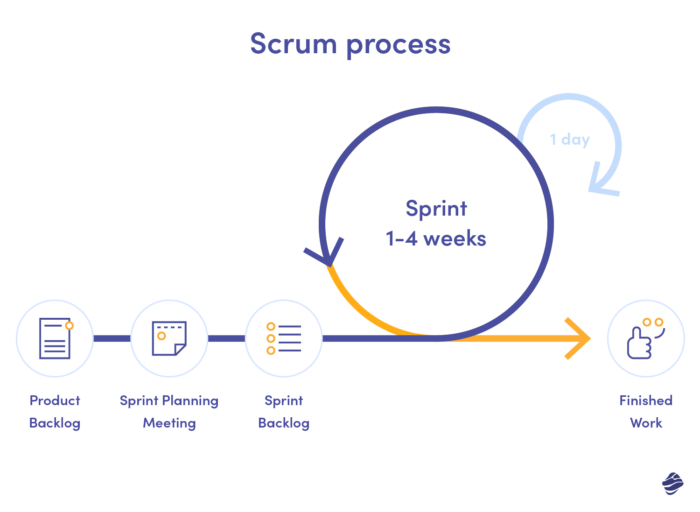
\includegraphics[width=0.75\textwidth]{images/scrum-overview}
    \caption{Overview of the Scrum framework.}
    \label{fig:scrum}
\end{figure}

\subsection{Why Scrum?}
Scrum was preferred over more rigid methodologies, such as Waterfall or the
V-Model, for several reasons that match the nature of this project.
\begin{itemize}
    \item \textbf{High research uncertainty}: building five
    artificial-intelligence agents involves frequent experimentation with
    models, datasets and architectures whose outcomes cannot be planned in
    detail months ahead. Sprints absorb this uncertainty through
    iteration-level re-planning.
    \item \textbf{Continuous feedback loop}: sprint reviews expose
    intermediate prototypes to the academic and industrial supervisors,
    which lets early misalignments be corrected before they propagate.
    \item \textbf{Alignment with the bootcamp cadence}: the Talan bootcamp
    itself follows a one-week-per-topic format with end-of-week defences,
    which integrates naturally with the Scrum sprint rhythm.
    \item \textbf{Visibility on progress}: a maintained backlog and a
    burndown chart give the supervisors a quantitative view of the work
    completed and of the remaining scope, which is critical under a fixed
    academic deadline.
    \item \textbf{Inspect-and-adapt culture}: retrospectives encourage
    explicit reflection on what worked at each sprint and support the
    continuous improvement of personal engineering practices throughout the
    internship.
\end{itemize}
The project relied on two-week sprints, a backlog hosted in a
project-management tool, weekly synchronisations with the supervisors and
end-of-sprint reviews that produced demonstrable artefacts.

\section{Data-Science Methodology}
The artificial-intelligence components of the platform --- the TAPJFNN
matching ranker, the candidate--skill graph neural network and the
supervised fine-tuning of the conversational large language model ---
were developed under the \textbf{CRISP-DM} (Cross-Industry Standard
Process for Data Mining) methodology. CRISP-DM organises a data-science
project around six iterative phases that together cover the lifecycle
from the business question to the deployment of the trained model.
Figure~\ref{fig:crispdm} illustrates its cyclic structure
\citeURL{crispdmDiagram}.

\begin{figure}[H]
    \centering
    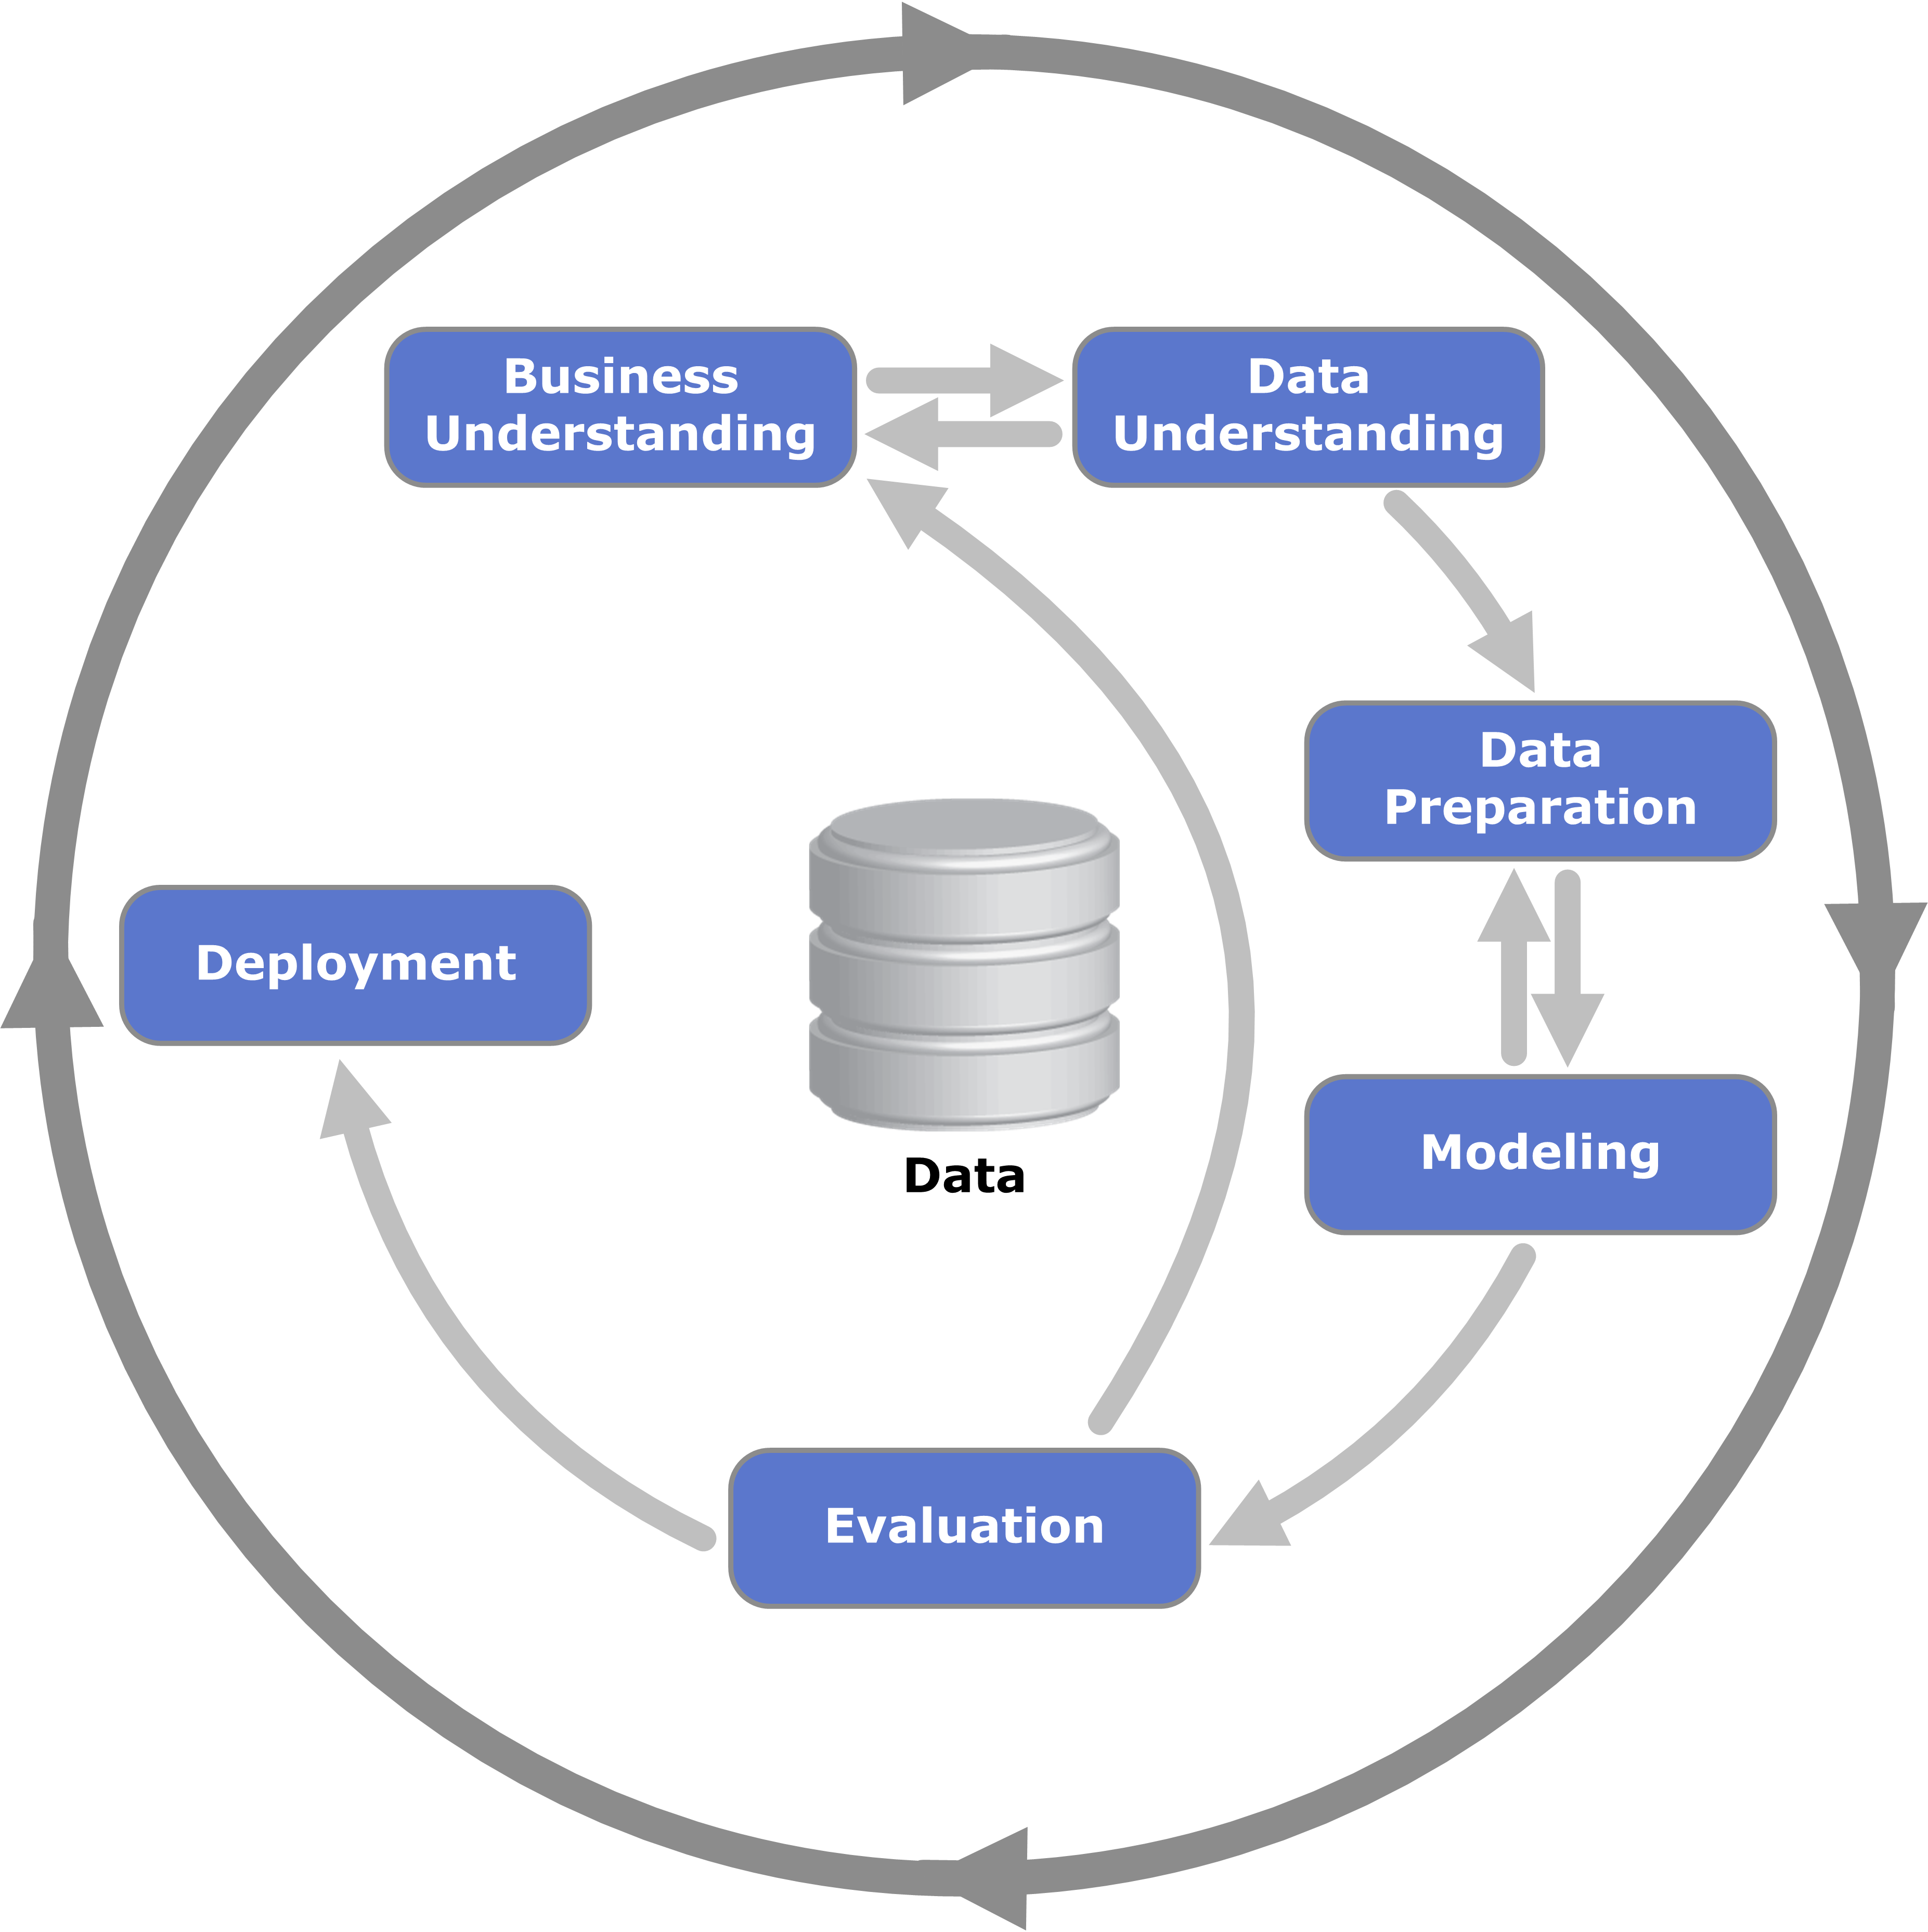
\includegraphics[width=0.55\textwidth]{images/crispdm}
    \caption{Overview of the CRISP-DM lifecycle.}
    \label{fig:crispdm}
\end{figure}

\subsection{Why CRISP-DM?}
CRISP-DM was preferred over a purely engineering-driven workflow because
the AI components of HireFlow are data-bound and require explicit handling
of dataset assumptions, leakage controls, distribution shift and offline
evaluation. The same six phases were applied independently to each of the
three models, while still leaving room for the back-and-forth between
modelling and data preparation that is typical of deep-learning iteration
cycles.
\begin{itemize}
    \item \textbf{Business understanding}: each model was framed against a
    concrete recruiter-facing metric --- top-$k$ matching accuracy for
    TAPJFNN, skill-graph link prediction for the GNN,
    instruction-following quality and JSON schema adherence for the
    fine-tuned LLM --- before any data was collected.
    \item \textbf{Data understanding}: exploratory analyses surfaced class
    imbalance, missing-skill artefacts and recruiter-bias signals that
    would otherwise have leaked into the trained models.
    \item \textbf{Data preparation}: deduplication, anonymisation,
    train/validation/test stratification by job family and balanced
    negative-sampling strategies were defined per model.
    \item \textbf{Modelling}: each model was iterated under shared
    experiment-tracking conventions, with hyper-parameter sweeps logged
    centrally for reproducibility.
    \item \textbf{Evaluation}: held-out metrics were complemented by an
    offline replay against historical hiring decisions and by a fairness
    audit on protected attributes.
    \item \textbf{Deployment}: each trained artefact was wrapped behind
    the same FastAPI agent contract, versioned and shadow-tested before
    replacing the previous model in production.
\end{itemize}
The combination of Scrum at the project level and CRISP-DM at the
data-science level allowed managerial agility and methodological rigour
to coexist throughout the internship.

\section{Conclusion}
This chapter introduced the host organisation, motivated the project,
surveyed existing tooling, presented the proposed multi-agent platform
and described the project-management (Scrum) and data-science (CRISP-DM)
methodologies under which the work was conducted. The remaining chapters
detail the technical foundations, design and experimental validation of
each agent.
